\section{Methodology}
\label{sec:methodology}

\subsection{Framework and Traffic Evidence}
\label{sec:framework-evidence}

The proposed framework separates grounded exploration, LLM-guided refinement,
and simulation-based decision making.  As shown in Figure~\ref{fig:framework}, an
unmodified SUMO scenario is first simulated to establish a baseline.  A
deterministic diagnosis module extracts traffic measurements and a compact
bottleneck-centered subgraph.  A seeded grounded sampler initializes one
intervention from each control family, which is validated and evaluated
independently.  A
feedback-guided beam then sends measured outcomes back to the responsible
specialists for one LLM-selected local refinement.  The remaining budget is
used for compatible two-action bundles.  If no unseen legal refinement or
compatible bundle is available, the budget remains unused rather than being
filled by a deterministic backfill policy.  The best measured candidate is
selected subject to explicit safety constraints.  The LLM supplies grounded
search directions, whereas the orchestrator enumerates legal local alternatives
and SUMO provides the decision evidence.

\begin{figure}[htbp]
    \centering
    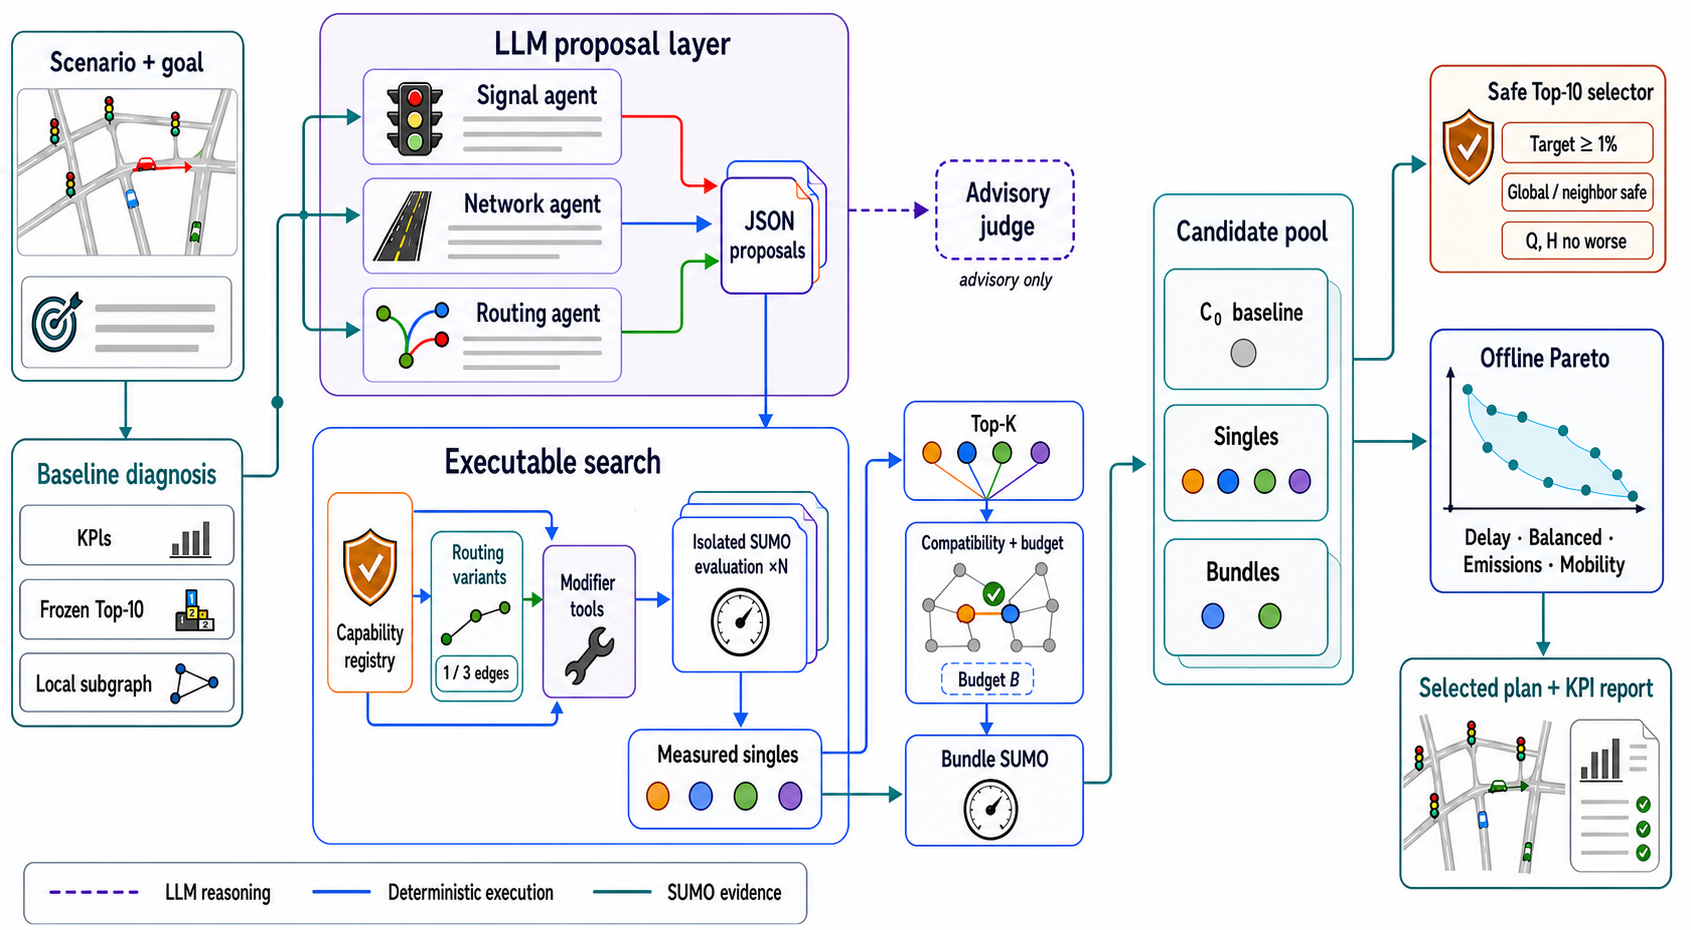
\includegraphics[width=\linewidth]{figures/framework_code_ai_simplified.png}
    \caption{Simulation-grounded multi-agent traffic optimization framework.
    Grounded sampling initializes diverse interventions; specialist LLM agents
    refine measured parents, after which compatible actions may be composed
    before constrained final selection.}
    \label{fig:framework}
\end{figure}

The input consists of a SUMO network, an OD-demand file, and a simulation
configuration.  The baseline run produces vehicle-level \texttt{tripinfo} and
60-second edge measurements.  The diagnosis aggregates speed, density,
occupancy, waiting time, time loss, and traffic exposure.  For each edge $e$, it
computes

\begin{equation}
\begin{split}
C_e ={}& 0.35(1-r_e)
       +0.25\,\phi(\rho_e;35)
       +0.20\,\phi(o_e;30) \\
     & +0.10\,\phi(L_e;300)
       +0.10\,\phi(W_e;300),
\end{split}
\label{eq:congestion-score}
\end{equation}

where $r_e$ is the observed-to-permitted speed ratio, $\rho_e$ is density,
$o_e$ is occupancy, $L_e$ and $W_e$ are accumulated time loss and waiting time,
and $\phi(x;h)=\min(1,\max(0,x/h))$.  To reduce sensitivity to microscopic
network segmentation, non-internal edges shorter than 10 m are excluded before
ranking.  The ten highest-scoring eligible edges define the baseline-frozen
Top-10 target set.  Up to five diagnosed edges also seed a
one-hop local subgraph, limited to 80 edges, that provides agents with valid
neighbor, junction, and traffic-light identifiers without inserting the full
network XML into their prompts.

The score grounds proposal generation rather than evaluating policies; final
decisions use simulated outcomes.  Freezing the Top-10 set prevents a moving
target in which an intervention appears effective merely because congestion is
shifted elsewhere.  The local subgraph retains enough topology to identify
contiguous corridors and nearby controllers while limiting prompt length.

\subsection{Optimization Problem Formulation}
\label{sec:optimization-formulation}

The optimization object is an executable intervention plan, not an LLM's prose
recommendation or predicted KPI value.  We represent a plan as

\begin{equation}
\mathbf{x}=
\left(x^{\mathrm{sig}},x^{\mathrm{net}},x^{\mathrm{route}}\right)
\in\mathcal{X}_{\mathrm{cap}},
\label{eq:decision-vector}
\end{equation}

where an inactive component is denoted by $\emptyset$.
$x^{\mathrm{sig}}$ specifies a traffic-light controller and its derived
fixed-time phase plan; $x^{\mathrm{net}}$ specifies either a corridor-speed
change, an edge removal, or a one-way conversion together with its target and
discrete parameter; and $x^{\mathrm{route}}$ specifies an avoided edge and the
rerouted fraction.  The capability-grounded domain
$\mathcal{X}_{\mathrm{cap}}$ contains only schema-valid actions, scenario-valid
identifiers, and supported discrete values.  A single plan activates one
component, while a compatible bundle activates at most two components.  This
cardinality limit and the compatibility rules prevent the optimizer from
combining conflicting edits or changing the same control family twice.

Let the deterministic SUMO evaluation map be

\begin{equation}
\mathcal{S}(\mathbf{x})=
\left(L_{\mathcal{T}},L_{\mathcal{N}},D,Q,H,E,V\right),
\label{eq:simulator-response}
\end{equation}

where $L_{\mathcal{T}}$ is total time loss on the baseline-frozen Top-10 edges,
$L_{\mathcal{N}}$ is time loss on their one-hop neighbors, $D$ is network-wide
mean vehicle time loss, $Q$ is throughput, $H$ is the teleport count, $E$ is
total $\mathrm{CO}_2$, and $V$ is mean speed.  Superscript $0$ below denotes
the response of the unmodified scenario $\mathbf{x}_0$.  We also define
$A(\mathbf{x})=1$ when all demand records and edge-level OD pairs are
preserved.  The primary optimization problem is

\begin{equation}
\begin{aligned}
\mathcal{F}=\{\mathbf{x}\in\mathcal{X}_{\mathrm{cap}}:\quad
&A(\mathbf{x})=1,\quad
L_{\mathcal{T}}(\mathbf{x})\leq0.99L_{\mathcal{T}}^0,\\
&D(\mathbf{x})\leq1.01D^0,\quad
L_{\mathcal{N}}(\mathbf{x})\leq1.05L_{\mathcal{N}}^0,\\
&Q(\mathbf{x})\geq Q^0,\quad H(\mathbf{x})\leq H^0\},\\
\mathbf{x}^*&=
\begin{cases}
\arg\min_{\mathbf{x}\in\mathcal{F}}L_{\mathcal{T}}(\mathbf{x}),
&\mathcal{F}\neq\emptyset,\\
\mathbf{x}_0,&\mathcal{F}=\emptyset.
\end{cases}
\end{aligned}
\label{eq:top10-constrained-selection}
\end{equation}

Thus, the optimized quantity is frozen-bottleneck time loss.  The 1\% Top-10
requirement is an acceptance threshold; global delay and neighboring time loss
are bounded spillover constraints; and demand integrity, throughput, and
teleports are operational constraints.  Emissions and speed are reported as
secondary outcomes and enter only the offline Pareto dominance audit.
This separation prevents the legacy weighted score or an LLM-predicted effect
from being mistaken for the objective used by the primary optimizer.

\subsection{Grounded Random Initialization}
\label{sec:grounded-proposals}

The diagnosis defines a discrete search space over the baseline-frozen
objective edges.  Before sampling, the executable capability validator removes
non-optimizable controllers, missing reverse-edge pairs, detectable local
topology violations, and malformed controls.  This pre-execution check confirms
that a candidate is supported and locally well formed; complete demand and OD
preservation are checked again after the modification is materialized.  Using
the recorded case seed, the primary optimizer samples one validator-confirmed
proposal from each available specialist family in round-robin order.  The
signal family selects an evidenced controller for fixed-time green-split
optimization while preserving phase states and transition intervals.  The
network family samples a legal corridor-speed, edge-removal, or one-way action;
corridor speed factors belong to $\{0.7,0.8,0.9\}$.  The initial routing family
uses a one-edge trust region and chooses

\begin{equation}
    \alpha\in\{0.25,0.50,0.75,1.00\}
\end{equation}

as the rerouted fraction.  The first three samples are exactly the prefix of
the grounded-random baseline generated with the same seed.  Thus, the feedback
ablation starts from identical initial actions and differs only in how the
remaining simulation budget is allocated.  A pure specialist-LLM initialization
is retained as an ablation, but is not the primary hybrid configuration.

Only vehicles whose
reference routes traverse a selected edge are eligible, and avoidance is soft
so that endpoints and unavoidable connections remain valid.  Unselected
vehicles retain their reference routes, and every modified demand file must
preserve all records and OD pairs.

Specialization prevents an agent from editing the entire scenario.  As
illustrated in Figure~\ref{fig:intervention-mechanisms}, signal proposals change
green allocation without altering phase states or transitions; corridor edges
are resolved deterministically from an evidenced anchor; and the routing
utility, rather than the LLM, selects eligible vehicles and verifies route
connectivity.  The model therefore supplies high-level search choices, while
deterministic code performs the network edits.

\begin{figure}[htbp]
    \centering
    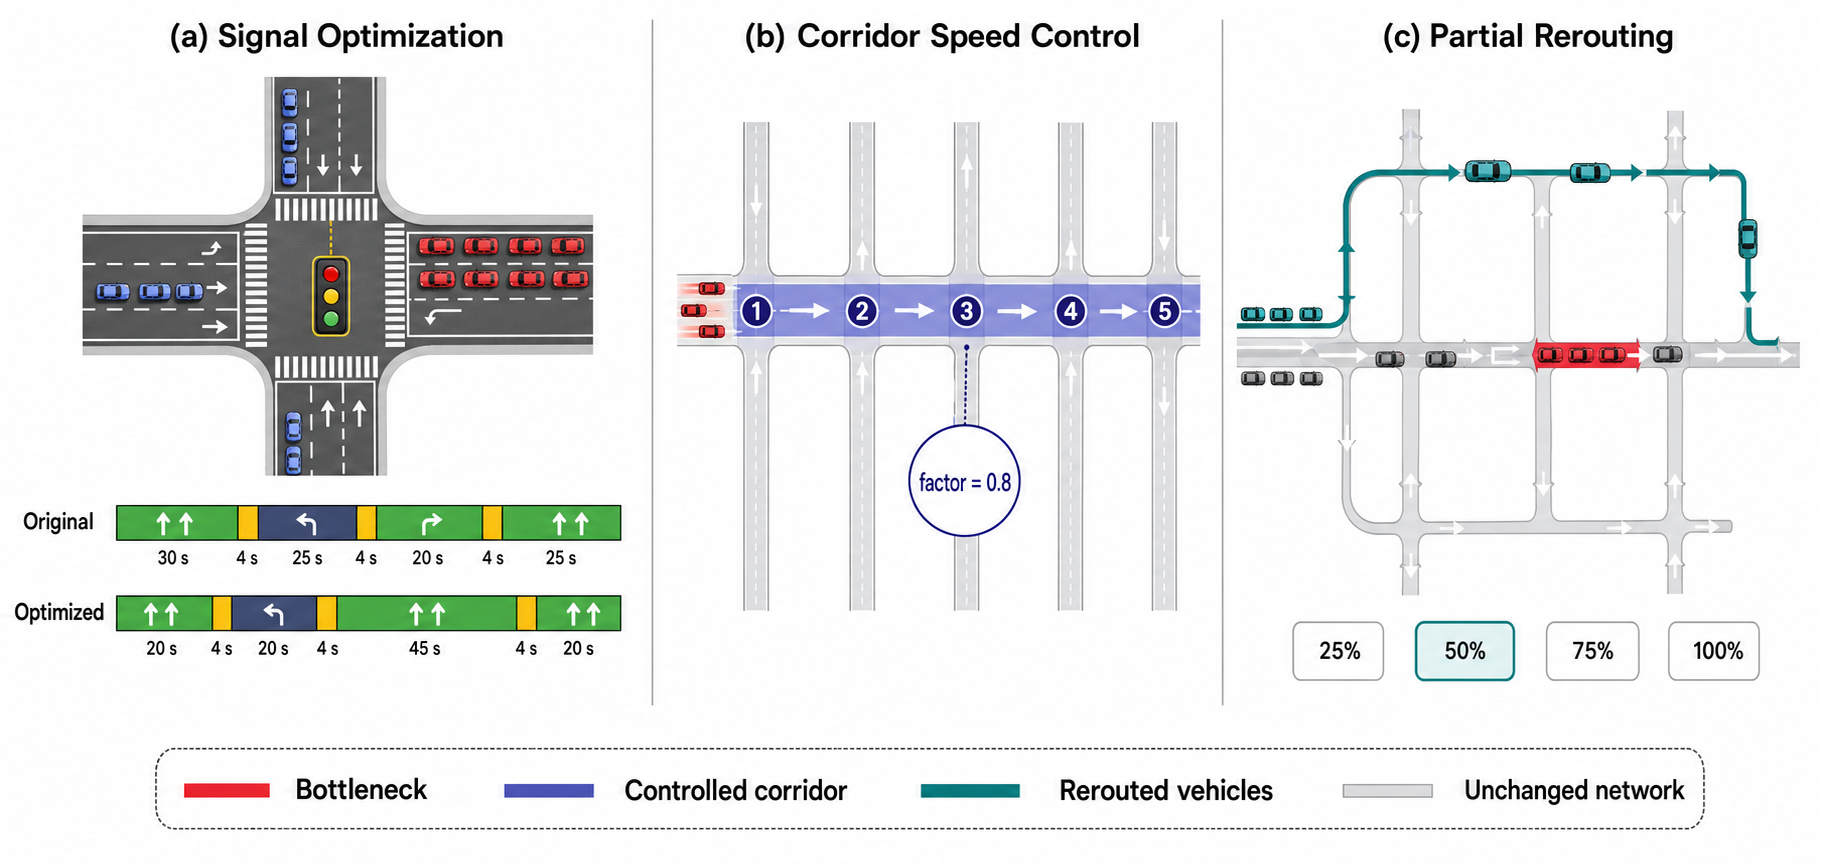
\includegraphics[width=\linewidth]{figures/intervention_mechanisms.png}
    \caption{Intervention mechanisms supported by the optimizer: fixed-time
    signal green-split adjustment, corridor-level speed control, and partial
    rerouting around a diagnosed bottleneck.  Grounded initialization or an LLM
    feedback specialist selects high-level targets and parameters, while
    deterministic utilities apply the corresponding SUMO modifications.}
    \label{fig:intervention-mechanisms}
\end{figure}

Each initializer returns one structured proposal containing an executable action,
target, parameters, evidence references, expected effects, and risks.  Before
execution, a deterministic capability registry checks that the action is
implemented, required artifacts and parameters are present, and every edge or
traffic-light identifier exists in the scenario.  Invalid fractions,
placeholders, unsupported operations, and incomplete proposals are rejected.
An LLM judge may provide an advisory comparison, but neither its recommendation
nor an agent's predicted benefit controls final selection.

Validation is performed in two stages.  Schema validation first checks the
proposal type, required fields, numeric ranges, and argument names.  Scenario
validation then binds those arguments to the current SUMO files and checks
identifier existence and action-specific preconditions.  Expected effects are
normalized to the categories \texttt{improve}, \texttt{unchanged},
\texttt{worsen}, and \texttt{unknown} for logging and interpretation.  These
claims are never substituted for observed KPIs.  This design prevents a fluent
but unsupported proposal from entering the expensive simulation stage and
provides a trace from every executable modification back to baseline evidence.

\subsection{Simulation-Grounded Candidate Search}
\label{sec:candidate-search}

Every validated random-initial proposal is applied to an isolated copy of the
baseline scenario and evaluated through a complete SUMO simulation.  All
candidates start from identical baseline artifacts, and a failed candidate does
not affect the remaining evaluations.  The resulting vehicle- and edge-level
outputs are processed using the same definitions as the baseline, producing
measured KPIs and explicit constraint violations for each intervention.

The feedback-guided configuration then retains a feasible-first beam
$\mathcal{B}_{t}$ of width $b$.  Ties are resolved by measured objective value,
while role diversity prevents minor variants from one intervention family from
occupying the entire beam.  For every parent $c\in\mathcal{B}_{t}$, its
specialist receives the measured KPI vector, Top-10 improvement, global and
neighbor changes, and failed constraints.  Deterministic code first enumerates
a finite catalog $\mathcal{M}(c)$ of unseen, validator-confirmed mutations that
retain the action and change exactly one decision argument.  The specialist
then selects one mutation identifier $m(c)\in\mathcal{M}(c)$ using the measured
feedback; it cannot introduce a new identifier or numeric value.  The update is

\begin{equation}
\mathcal{C}_{t+1}=\mathcal{C}_{t}\cup
\{m(c):c\in\mathcal{B}_{t}\},\qquad
\mathcal{B}_{t+1}=\operatorname{Top}_{b}^{\mathrm{feas,div}}
(\mathcal{C}_{t+1}),
\label{eq:feedback-beam-update}
\end{equation}

where every selected mutation is revalidated and re-simulated before it can
enter the next beam.  An invalid catalog selection receives one LLM repair
attempt.  Action changes, multi-argument rewrites, and previously tested
duplicates are rejected without consuming the SUMO budget.  The initial
version uses two proposal rounds and beam width $b=2$; setting the number of
rounds to one recovers the one-shot proposal baseline.  Candidate simulation
budget that cannot be used because a refinement is invalid or duplicated
remains unused; all feedback-guided mutations are chosen by the responsible LLM
specialist from the program-generated legal catalog.  Figure~\ref{fig:llm-feedback-optimization}
summarizes this grounded generate--evaluate--refine cycle.

\begin{figure*}[!ht]
  \centering
  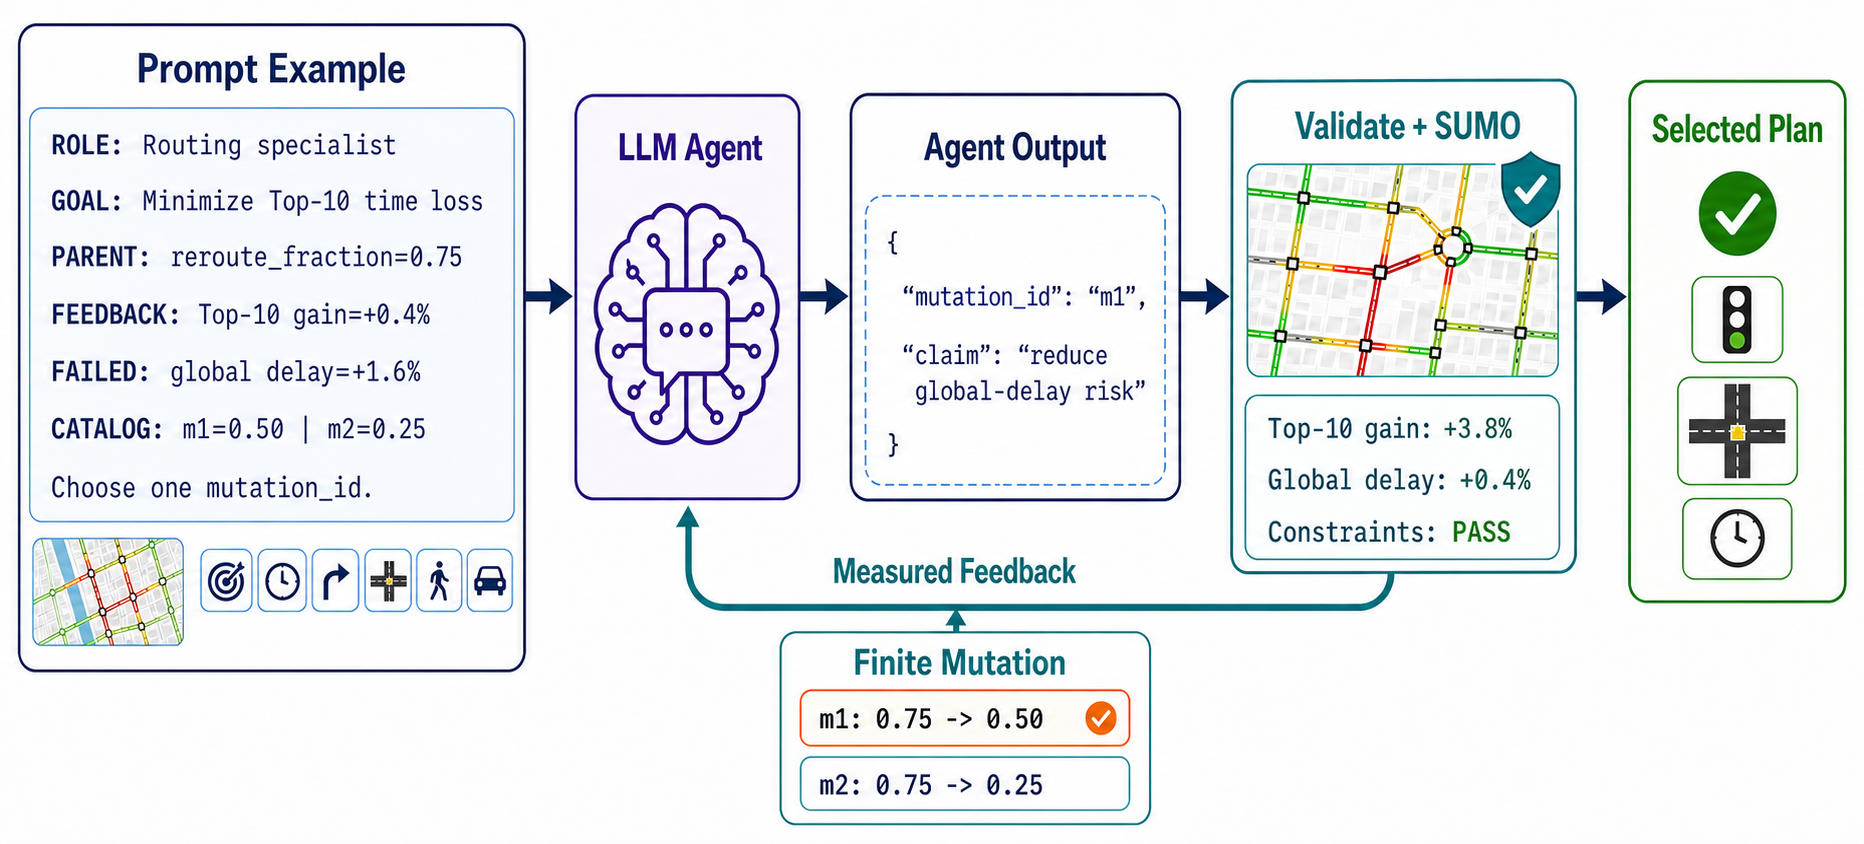
\includegraphics[width=0.96\textwidth]{figures/llm_feedback_optimization_v2.png}
  \caption{Illustrative LLM feedback-refinement example.  The prompt provides
  the role, objective, simulated parent outcome, failed constraint, and a
  validator-generated mutation catalog.  The agent returns only a legal
  mutation identifier; the modified plan is independently revalidated and
  simulated before selection.  Numeric values are illustrative.}
  \label{fig:llm-feedback-optimization}
\end{figure*}

After feedback refinement, the system retains the top $K$ single candidates and
enumerates compatible pairs within a remaining simulation budget $B$.  A bundle contains at most one action from each
intervention family, and actions that conflict on the same edge or controller
are rejected.  Compatible actions are applied in the order

\begin{equation}
\text{topology}\rightarrow\text{speed}\rightarrow
\text{routing}\rightarrow\text{signal},
\label{eq:bundle-order}
\end{equation}

so each action is rebound to the artifacts produced by the preceding step.
The complete bundle is then re-simulated rather than scored by adding its
constituents' predicted or isolated effects.  Successfully evaluated singles
and bundles form the final candidate pool $\mathcal{C}$.

The beam width, Top-$K$ filter, and bundle budget control the number of
additional SUMO runs.  Singles are ordered using their measured performance, after which the
compatibility checker excludes repeated intervention families and conflicting
targets, such as speed modification and soft avoidance of the same edge.  The
sum of single-candidate scores is used only to prioritize which compatible
pairs receive the limited simulation budget.  It is not treated as the bundle's
performance because two individually useful actions can reinforce, cancel, or
shift the effects of one another.  The bundle run therefore captures interaction
effects that cannot be inferred reliably from the isolated evaluations.  In
the reported experiments, $K=4$, at most two bundles are simulated, and the
total candidate budget is capped at seven SUMO evaluations per case; these
settings apply equally to the LLM and non-LLM proposal-source conditions.

\subsection{Constrained Final Selection}
\label{sec:constrained-selection}

Demand preservation is a hard feasibility requirement.  A candidate is
discarded if it changes the number of demand records or any OD pair.  Throughput
is measured against the original source demand as
$Q=N_{\mathrm{completed}}/N_{\mathrm{source}}$, preventing an intervention from
appearing beneficial by silently removing difficult trips.

This formulation avoids assigning an arbitrary fixed delay penalty to
unfinished vehicles.  Instead, incomplete service is exposed directly through
throughput and teleport constraints.  Delay and time
loss are computed from the vehicles and edge measurements actually reported by
SUMO, while demand preservation ensures that the denominator cannot be changed
by an intervention.  The same aggregation code and simulation horizon are used
for the baseline and every candidate.

Equation~\ref{eq:top10-constrained-selection} is applied only to measured SUMO
outcomes.  An intervention must therefore produce at least a 1\% bottleneck
improvement, may increase global delay by at most 1\%, may increase neighboring
time loss by at most 5\%, and cannot reduce throughput or increase teleports.
The unmodified scenario $\mathbf{x}_0$ acts as a no-operation guard.  For the
legacy scalar comparison only, candidates are ranked by

\begin{equation}
J_{\mathrm{legacy}}(c)=
0.50\frac{D(c)}{D(c_0)}+0.10\frac{E(c)}{E(c_0)}
-0.25\frac{Q(c)}{Q(c_0)}-0.15\frac{V(c)}{V(c_0)},
\label{eq:legacy-objective}
\end{equation}

where $E$ and $V$ denote $\mathrm{CO}_2$ and mean speed.  This legacy score is
not the primary selection rule.

The rule distinguishes target improvement from network-wide acceptability.
$L_{\mathcal{T}}$ tests whether the diagnosed bottlenecks improve,
$L_{\mathcal{N}}$ detects immediate spillover, and $D$ prevents a local gain
from being purchased through worse overall travel conditions.  Throughput and
teleports serve as operational safeguards.  The 1\% threshold suppresses
negligible changes that may arise from stochastic simulation variation, while
the neighbor tolerance permits limited redistribution around a bottleneck.  If
several candidates pass all requirements, minimizing frozen Top-10 time loss
keeps the final decision aligned with the stated local optimization objective.

\subsection{Pareto Dominance Audit}
\label{sec:pareto-method}

To check whether the delay-oriented selector discards an unambiguously better
candidate, an offline analysis examines each saved candidate pool using four
baseline-relative gains:

\begin{equation}
\begin{aligned}
g_T(c) &= 1-\frac{L_{\mathcal{T}}(c)}{L_{\mathcal{T}}(c_0)}, &
g_D(c) &= 1-\frac{D(c)}{D(c_0)},\\
g_E(c) &= 1-\frac{E(c)}{E(c_0)}, &
g_V(c) &= \frac{V(c)}{V(c_0)}-1.
\end{aligned}
\label{eq:pareto-gains}
\end{equation}

Candidates must preserve complete demand, throughput, teleports, and the global
and neighbor bounds in Equation~\ref{eq:top10-constrained-selection}.  A
candidate is Pareto-optimal when no other feasible candidate is at least as
good in all four gains and strictly better in one.  The baseline remains in
every pool.  This audit requires no additional LLM calls or SUMO runs and does
not alter the selected plan: it reports whether the plan chosen by the primary
Top-10 delay objective lies on the measured Pareto front.  Consequently, no
manually weighted preference profiles are introduced into the optimizer.
